\section{Theory: Two Kinds of Robustness}
\label{sec:theory}

\subsection{Overview: collective versus local questions}
\label{sec:theory-overview}

The experiments in this report ask two different questions of the same
damaged graph. The structural question is whether a node still belongs to the
largest connected component. The functional question is whether one particular
drug--disease query still has a typed path of at most $L$ hops. These questions
look similar, but they belong to two different kinds of mathematics.

Membership of the giant component is a \emph{collective} property. Whether a
node is connected to the giant component depends on its neighbours, on their
neighbours, and so on without limit. Percolation theory handles this with a
self-consistency equation, solved with the generating functions of the course,
and the solution has a threshold: below a critical retention probability the
giant component vanishes. A two-hop query is a \emph{local} property. It
depends on a fixed handful of edges, so its survival probability is a finite
polynomial in the retention probability, with no self-consistency equation and
no threshold. The query horizon $L$ interpolates between the two cases.

Table~\ref{tab:theory-map} summarises the predictions developed below. Each is
computed from the intact graph and contains no fitted parameter. Each assumes
that damage is \emph{blind}, that is, independent of the graph structure.
Section~\ref{sec:prediction} tests where this assumption holds and where
targeted damage breaks it.

\begin{table}[!htbp]
\centering
\small
\caption{Theoretical predictions used in this report. Edge retention is
$p=1-f$, and node retention is $\phi=1-f$. The last column gives the largest
difference from the reference simulation over the stated range.}
\label{tab:theory-map}
\begin{tabular}{@{}p{0.20\linewidth}p{0.20\linewidth}p{0.25\linewidth}p{0.27\linewidth}@{}}
\toprule
Observable & Depends on & Prediction & Agreement with simulation \\
\midrule
Giant component $S$ & Unbounded number of edges (collective) & GF self-consistency, Eqs.~\eqref{eq:gf-bond}--\eqref{eq:gf-site}; threshold $p_c$ & Same-degree random graphs: $\le 0.0012$. PrimeKG random removal, $f\le0.90$: $\le0.0011$ (edges), $\le0.0033$ (nodes). Degree attack: up to 0.11 \\
Two-hop success $R_2$ & $2m$ fixed edges (local) & Reliability polynomial $1-G_m(1-p^2)$, Eq.~\eqref{eq:r2} & $\le 0.001$ against 5,000 fresh damage orders (edges and nodes) \\
Unlimited-hop success $R_\infty$ & Endpoint links plus PPI giant component & GF attachment, Eq.~\eqref{eq:rinf}; min-cut form, Eq.~\eqref{eq:mincut} & $\le 0.009$ for all $f$; min-cut form $\le 0.005$ for $f\le 0.80$ \\
\bottomrule
\end{tabular}
\end{table}

\subsection{Global connectivity: generating-function percolation}
\label{sec:theory-gf}

Let $p_k$ be the empirical degree distribution of the structural graph, with
generating function $g_0(z)=\sum_k p_k z^k$. Following an edge reaches a node
whose remaining (excess) degree has generating function
$g_1(z)=g_0'(z)/g_0'(1)$ \cite{newman2001random}. Let $u$ be the probability that an edge does not lead
to the giant component. Under random edge removal with retention $p$, an edge
fails to lead there either because it was removed, or because it survived but
none of the other edges of the node it reaches leads there:
\begin{equation}
u = 1-p+p\,g_1(u), \qquad S_{\mathrm{bond}}(p)=1-g_0(u).
\label{eq:gf-bond}
\end{equation}
For random node removal with retention $\phi$, the same argument gives
\begin{equation}
u = 1-\phi+\phi\,g_1(u), \qquad S_{\mathrm{site}}(\phi)=\phi\,[1-g_0(u)].
\label{eq:gf-site}
\end{equation}
A nontrivial solution $u<1$ exists only when $p\,g_1'(1)>1$. This is the
Molloy--Reed condition \cite{molloy1995critical}, which gives the threshold
\begin{equation}
p_c=\frac{\langle k\rangle}{\langle k^2\rangle-\langle k\rangle}.
\label{eq:pc}
\end{equation}
For targeted removal of the highest-degree nodes we use the
generalisation of Callaway et al.~\cite{callaway2000network}. Let
$\phi_k$ be the probability that a node of degree $k$ survives. Then
$f_0(z)=\sum_k p_k\phi_k z^k$ and $f_1(z)=f_0'(z)/\langle k\rangle$, and the
giant component follows from $u=1-f_1(1)+f_1(u)$ and $S=f_0(1)-f_0(u)$. Nodes
at the cut-off degree are retained in the proportion that removes exactly
$\mathrm{round}(fN)$ nodes, so ties need no arbitrary ordering.

These equations describe an uncorrelated, locally tree-like random graph with
the observed degree sequence. They know nothing else about PrimeKG. Before
comparing them with PrimeKG, we checked them on ten random graphs built by matching
the stubs of the same degree sequence (self-loops removed). The largest difference from simulation
was 0.0012 for bond removal, 0.0011 for site removal and 0.0010 for the degree
attack up to $f=0.5$. The one exception is the attack at $f=0.6$, where the
theory has just crossed its threshold and finite-size effects leave a small
remnant. This check tests our code, not PrimeKG. On PrimeKG itself, the bond
and site predictions stay within 0.0011 and 0.0033 of the ten-seed means for
$f\le0.90$; the bond difference grows to 0.015 at $f=0.97$
(Section~\ref{sec:random-failure}). The degree attack is different:
the real graph lies up to 0.11 below the prediction. Section~\ref{sec:theory-null}
identifies the structure that causes this gap.

The protein--protein interaction (PPI) layer is very heterogeneous, so
$\langle k^2\rangle$ is large and Eq.~\eqref{eq:pc} gives
$p_c\approx0.0062$ for the PPI subgraph of the standard graph. The value is
0.0053 for the whole standard graph. Random edge removal must therefore delete
more than 99\% of edges before the giant component disappears. Our scan stops
at $f=0.99$, so we do not claim to have measured this threshold. The
practical consequence is that, under random damage, global connectivity is
almost the last thing to fail.

\subsection{Two-hop retrieval: a reliability polynomial}
\label{sec:theory-r2}

A two-hop query $(d,s)$ with $m$ shared proteins $x_1,\dots,x_m$ has $m$ routes
$d\!-\!x_i\!-\!s$. Route $i$ survives only if both of its edges survive. The
query succeeds if at least one route survives. Logically, each route is an AND
of two edges, and the query is an OR of $m$ routes. In reliability theory this
is a series--parallel network, the structure Moore and Shannon used to build
reliable circuits from unreliable relays \cite{moore1956reliable}.

Two routes through different proteins share no edge, because
$\{d\!-\!x_i, x_i\!-\!s\}$ and $\{d\!-\!x_j, x_j\!-\!s\}$ are disjoint for
$i\neq j$. Every endpoint pair in our graphs carries exactly one relation
($\texttt{pairs\_with\_multiple\_relations}=0$, Section~\ref{sec:data}), so
semantic and structural edges coincide. When each edge survives independently
with probability $p$, the routes therefore fail independently, and
\begin{equation}
\Pr[\text{query succeeds}\mid m]=1-(1-p^2)^m.
\end{equation}
Averaging over the benchmark gives the two-hop success rate
\begin{equation}
R_2(p)=\sum_m P(m)\,\bigl[1-(1-p^2)^m\bigr]=1-G_m(1-p^2),
\qquad G_m(z)=\sum_m P(m)\,z^m,
\label{eq:r2}
\end{equation}
where $P(m)$ is the redundancy distribution of the queries and $G_m$ is its
probability generating function. For random node removal, the drug and the
disease must themselves survive, and route $i$ needs only protein $x_i$:
\begin{equation}
R_2^{\mathrm{node}}(\phi)=\phi^2\,\bigl[1-G_m(1-\phi)\bigr].
\label{eq:r2-node}
\end{equation}
The only input is $P(m)$, which is known before any damage. Our experiments
delete an exact number of edges rather than deleting each edge independently.
This changes Eq.~\eqref{eq:r2} only at order $1/E$, with $E=117{,}891$.

Equation~\eqref{eq:r2} makes three points that the simulations alone do not.
\begin{enumerate}[leftmargin=*,itemsep=2pt]
\item \textbf{No threshold.} $R_2$ is a polynomial of degree at most
$2m_{\max}$ in $p$, and it does not change as the graph grows. A giant
component depends on an unbounded number of edges, which is why $S(p)$ can
become singular as $N\to\infty$. Retrieval with a bounded hop limit cannot.
This is why the $S$ and $R_2$ curves in Figure~\ref{fig:ws3-structure-vs-retrieval}
have different shapes, not just different values.
\item \textbf{Redundancy means independent cycles.} Two routes close the cycle
$d\!-\!x_1\!-\!s\!-\!x_2\!-\!d$, and $m$ routes create $m-1$ independent
cycles. Each additional cycle multiplies the failure probability by the same
factor $1-p^2$. A single-path query has no cycle, so each of its edges is a
single point of failure and $R_2=p^2$. This explains why single-path success at
$f=0.5$ is close to $0.5^2=0.25$ (Section~\ref{sec:functional}).
\item \textbf{The benchmark composition sets the answer.} Because $R_2$ depends
only on $P(m)$, a benchmark with different redundancy would have a different
robustness curve on the same graph. Robustness is a property of the pair formed
by the network and its task.
\end{enumerate}

\subsection{The long-horizon limit $L\to\infty$}
\label{sec:theory-rinf}

Without a hop limit, a query succeeds when the drug's surviving target
proteins and the disease's surviving associated proteins are connected through
surviving PPI edges. If the PPI layer has a giant component, this is almost
always the case when both endpoints keep at least one link into it. Let $u$
solve Eq.~\eqref{eq:gf-bond} for the PPI subgraph alone. A protein $x$ with PPI
degree $k_x$ lies in the PPI giant component with probability
$\pi_x=1-u^{k_x}$. An endpoint $a$ with partner proteins $\mathcal{N}(a)$
attaches to the giant component with probability
$A_a=1-\prod_{x\in\mathcal{N}(a)}(1-p\,\pi_x)$, and
\begin{equation}
R_\infty(p)\approx\frac{1}{|Q|}\sum_{(d,s)\in Q}A_d\,A_s .
\label{eq:rinf}
\end{equation}
Against the mean over 600 fresh damage orders, Eq.~\eqref{eq:rinf} stays within
0.009 at every removal fraction from 0.05 to 0.99.

The equation explains why we did not see the collapse we had expected. The PPI
giant component is extremely robust. It still contains 75\% of proteins at
$f=0.90$, in agreement with the GF value 0.751. Long before it breaks, the
endpoints lose their own links. In this benchmark the binding constraint is the
drug side. The 476 drug--protein edges are 0.4\% of all relations, and 51 of the
74 drugs have a single target. For every one of the 200 queries, the drug--disease
edge connectivity $\lambda$ computed by maximum flow on the intact graph equals
the smaller endpoint degree. In 89.5\% of queries that endpoint is the drug,
$\lambda=1$ for 21.5\% of queries, and $\lambda\le3$ for 32\%. While the PPI
giant component is intact, a query therefore fails essentially when the
smaller endpoint loses all of its links, which gives the same form as
Eq.~\eqref{eq:r2}:
\begin{equation}
R_\infty(p)\approx 1-G_\lambda(1-p),
\label{eq:mincut}
\end{equation}
with the minimum cut $\lambda$ in place of the path count $m$, and $p$ in place
of $p^2$, because each cut edge is a single link. This form is within 0.005 of
simulation for $f\le0.80$. Beyond that it overestimates success (by 0.021 at
$f=0.90$), because the PPI giant component starts to shrink and
Eq.~\eqref{eq:rinf} is then needed. Up to $f=0.90$, more than 90\% of
$L=\infty$ failures are queries whose drug has lost every target, while the
disease side is still attached.

The two limits therefore have the same structure. Success is one minus the
generating function of a redundancy distribution, evaluated at the failure
probability of one redundant unit. What changes with the horizon is what
counts as a unit: a two-edge route at $L=2$, and a single cut edge at
$L=\infty$.

\subsection{Intermediate horizons: limited path percolation}
\label{sec:theory-limited}

For $2<L<\infty$, a query needs a surviving route of bounded length. This is
limited path percolation \cite{lopez2007limited}, which has no simple closed
form, so we measure it directly. We define the damage at which horizon $L$
starts to bind as the first $f$ at which $R_L$ falls 5 percentage points below
$R_\infty$. Over 600 fresh orders, this happens at $f\approx0.10$, $0.50$ and
$0.85$ for $L=2$, $3$ and $4$ (Figure~\ref{fig:d-phase}). Each additional hop
moves the binding point to heavier damage. Moving between the curves in
Figure~\ref{fig:d-phase} therefore moves retrieval from local reliability,
described by Eq.~\eqref{eq:r2}, towards global attachment, described by
Eqs.~\eqref{eq:rinf}--\eqref{eq:mincut}. These are smooth crossovers on a finite
graph, not phase transitions. The circles in Figure~\ref{fig:d-phase} mark our
5-point criterion, not a phase boundary.

\begin{figure}[!htbp]
  \centering
  \includegraphics[width=0.95\linewidth]{act2/primekg_5000_bfs_v1/fig_phase_diagram.pdf}
  \caption{Retrieval success as a function of edge removal fraction $f$ and hop
  limit $L$ (left; ten random edge-removal seeds), with the two analytic limits
  (right). The upper right panel compares $L=2$ with Eq.~\eqref{eq:r2}, and the
  lower right panel compares $L=\infty$ with Eq.~\eqref{eq:rinf}. Neither curve
  has a fitted parameter. Circles mark the first $f$ at which $R_L$ falls 5
  percentage points below $R_\infty$, computed from 600 fresh orders.}
  \label{fig:d-phase}
\end{figure}

\subsection{Why the degree attack beats the theory: a null-model test}
\label{sec:theory-null}

Under the fixed degree attack of Section~\ref{sec:targeted-attacks}, PrimeKG
fragments faster than the Callaway prediction. The giant component is 0.883
instead of 0.942 after removing 5\% of nodes, and 0.546 instead of 0.648 after
removing 30\%. The theory is exact on random graphs with the same degree
sequence (Section~\ref{sec:theory-gf}), so the gap must come from structure that
the degree sequence does not contain. To find which structure, we rewired the
standard graph in three ways that keep every node's degree, and hence B's fixed
degree ranking, unchanged:
\begin{itemize}[leftmargin=*,itemsep=2pt]
\item \textbf{Full rewiring} \cite{maslov2002specificity}: double-edge swaps
that ignore relation type. Only the degree sequence is kept.
\item \textbf{Typed rewiring}: swaps only within one relation, exchanging the
protein ends of drug--protein and disease--protein edges. Every node keeps its
degree in every relation type.
\item \textbf{2K rewiring}: swaps only between edge ends whose endpoints have
equal degree. This keeps the joint degree distribution, and therefore the
degree--degree correlations, but randomises everything else.
\end{itemize}
Each model was run five times with ten attempted swaps per edge, and every
rewired graph was checked to be simple and to have the original degree
sequence. Figure~\ref{fig:d-null} shows the results. The spread across
realisations is at most 0.007 for 2K rewiring and 0.015 for typed rewiring.
For full rewiring it reaches 0.046 only near the threshold, at $f\approx0.55$.

\begin{figure}[!htbp]
  \centering
  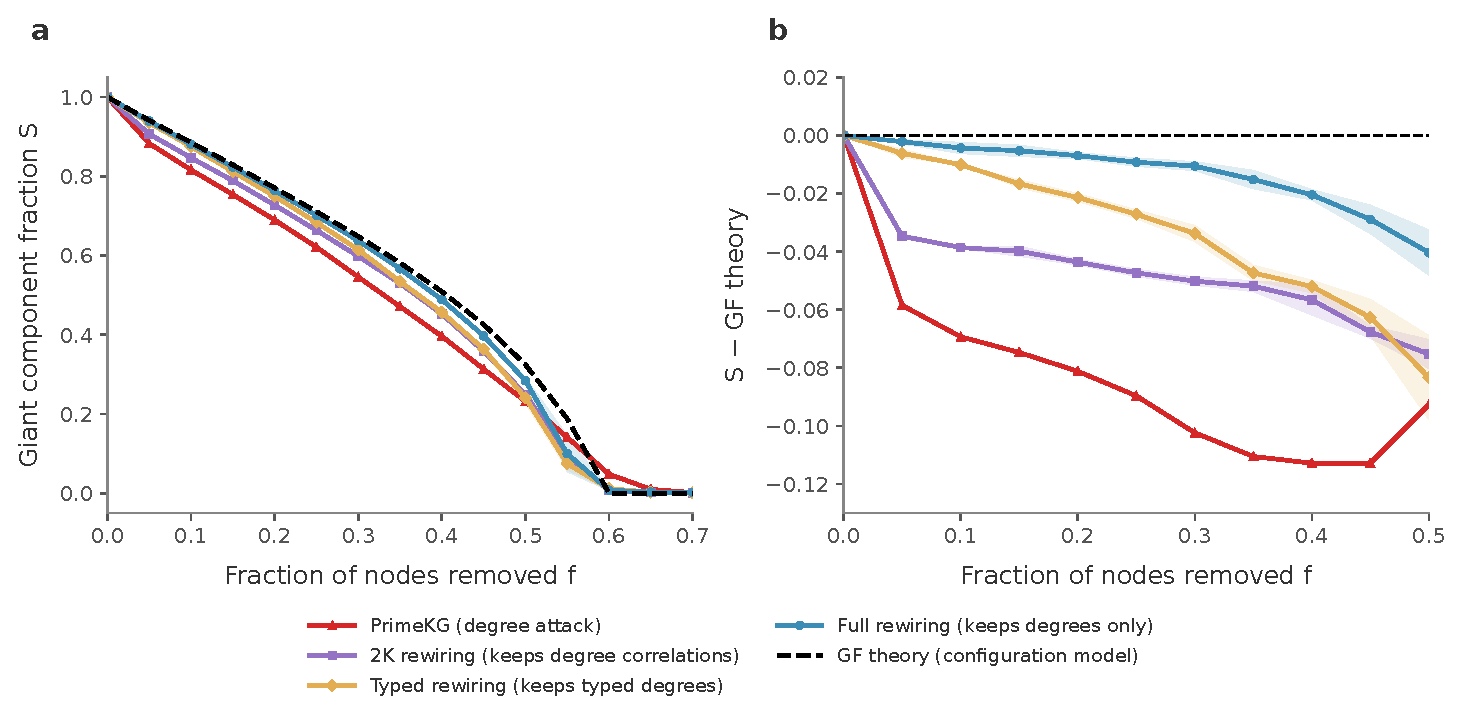
\includegraphics[width=\linewidth]{act1/primekg_5000_bfs_v1/fig_attack_null_model.pdf}
  \caption{Degree attack on PrimeKG and on three degree-preserving null models.
  (a) Giant component fraction. (b) Difference from the GF prediction for the
  configuration model. Null models are means over five realisations, and shading
  shows one sample standard deviation. All graphs share the degree sequence
  and the fixed degree ranking.}
  \label{fig:d-null}
\end{figure}

Fully rewired graphs follow the theory closely. Their remaining gap (0.011 at
$f=0.30$) comes from requiring a simple graph with a heavy-tailed degree
sequence. This requirement makes the graph mildly disassortative
(assortativity $r=-0.108$). Keeping the joint degree distribution recovers a
large part of the real fragility. PrimeKG is strongly disassortative
(degree assortativity $r=-0.153$ \cite{newman2002assortative}): nodes of degree at most 3 have neighbours of mean degree 486,
compared with 262 after full rewiring. These low-degree nodes hang from hubs, so
removing the hubs strands them. A 5\% attack isolates 6.7\% of all nodes in
PrimeKG, 4.3\% in the 2K graphs and 1.1\% in fully rewired graphs. Drugs show
the same effect most clearly. After the 5\% attack, 77\% of the surviving drugs
have no remaining neighbour in PrimeKG and 78\% in the 2K graphs, but only 26\%
after full rewiring. Typed rewiring lies in between, because the drug--protein
and disease--protein layers are disassortative by construction.

At $f=0.30$, the total gap of 0.102 splits approximately as follows. About 10\%
comes from the simple-graph constraint (theory to full rewiring). About 39\%
comes from degree correlations (full rewiring to 2K). The remaining 51\% comes
from structure beyond the joint degree distribution (2K to PrimeKG). This last
share is the largest. Plausible causes are clustering, disease modules and the
breadth-first sampling, which reaches peripheral nodes through hubs. We did not
separate these causes. The conclusion we can support is narrower but useful:
\emph{the configuration-model theory fails under attack because PrimeKG hangs its
low-degree entities, including most drugs, on its hubs}. The same hubs carry the
shared proteins of the retrieval queries. Section~\ref{sec:prediction-attack}
shows that this costs retrieval far more than it costs connectivity.
